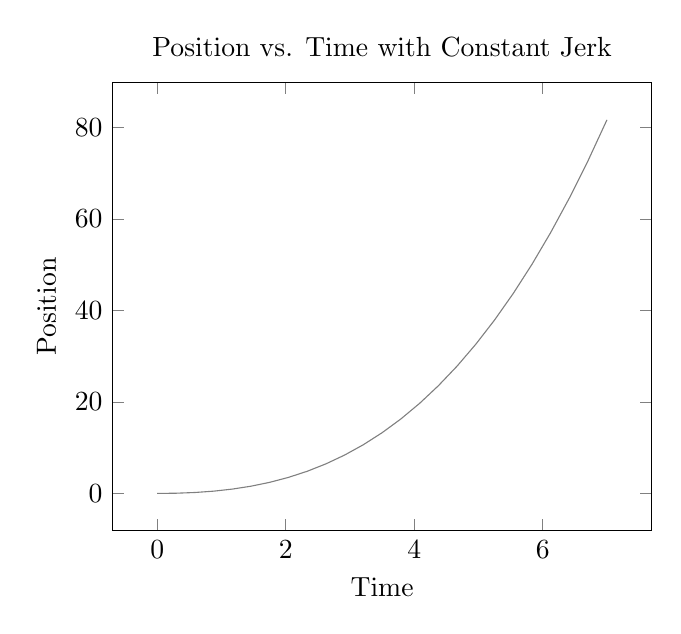
\begin{tikzpicture}
\begin{axis}[title = {Position vs. Time with Constant Jerk}, xlabel = {Time}, ylabel = {Position}, domain = 0:7]
\addplot[color=gray]{x^2/2+x^3/6};
\end{axis}
\end{tikzpicture}
\newline
The most natural question I had when learning elementary physics was, what happens kinematically and dynamically when the acceleration of an object we are examining is changing. The AP Physics Exam will only teach you about kinematics problems in which the acceleration is constant, but of course; in many real-world problems, the acceleration is changing. Sustaining constant acceleration requires quite a bit of energy especially when we consider the fact that friction exists. In order to work with non-constant acceleration problems, we can define \begin{equation}\vec{J}= \frac{d\vec{a}}{dt}\end{equation} where $\vec{J}$ is called jerk. Through the definitions of derivatives, we can show that jerk, while being equal to the first time-derivative of acceleration, is also equal to the second time derivative of velocity and the third time derivative of position. The most complex problem regarding the change of acceleration over time will be when we define the position of an object in linear space as a function $\vec{x}\left(t\right)$ where $\vec{x}\left(t\right)$ is a simple polynomial. Finding the velocity, acceleration, and jerk for this situation requires taking derivatives with respect to time. This is fairly simple and with enough practice will become a rote concept. I will not go over it more because it requires very little conceptual thinking. Perhaps more advanced is finding a velocity function for an object given an acceleration function $\vec{a}\left(t\right)$, and then finding a position  function using $\vec{v}\left(t\right)$. The important thing when doing these problems is to make sure we add a constant term to a function whenever we integrate over time. So in order to truly find a position function $\vec{v}\left(t\right)$ given an acceleration function $\vec{a}\left(t\right)$ we need to be given an initial value of $\vec{v}\left(t_0\right)$ at some  time $t_0$. This pair of $t_0$ and $\vec{v_0} \left(t\right)$ is called our initial condition. In differential equations, these initial conditions are critical. Quite frequently, we are told that initially, our body of interest is at rest. This is just another way of saying that our initial condition is given by $t_0=0$, $\vec{v_0}\left(0\right)=0$. So, for example, if we are given that a body is initially at rest and that $a\left(t\right)=t+1$. 

Note: In this example as in all others, the units will not match up as we assume that t is not 6 seconds but instead just 6 and $\vec{a}\left(t\right)$ is not 6 $\frac{m}{s^2}$ but rather only 6. However, when we use the acceleration as a function of time in an outside context, we must make sure to use the acceleration with the proper units as it can get quite confusing if we do not. 

We then have that \begin{equation}v\left(t\right)=6t+\frac{1}{2}t^2+C_1\end{equation} We can now plug in to find t. \begin{equation}6\left(0\right)+\frac{1}{2}\left(0\right)^2+C_1=0\end{equation} So $$C_1 = 0$$ and \begin{equation}v\left(t\right)=t+\frac{1}{2}t^2\end{equation} Next, we can try to find the change in position of the body as a function of time. If we are asked to find the change of a ball over time, this means we can assume that the ball is at position $\vec{x_0} = 0$ at time 0 because the change in position is 0 at time 0. So we now say that \begin{equation}x\left(t\right)=\frac{1}{2}t^2+\frac{1}{6}t^3+C_2\end{equation} However, we assumed that $x\left(0\right)=0$, so $0=0+0+C_2$. So $C_2=0$ and, finally, \begin{equation}x\left(t\right)=\frac{1}{2}t^2+\frac{1}{6}t^3\end{equation} Real world problems will not always be this trivial and sometimes the initial conditions will not be given conveniently at time and position being equal to 0. However, fundamentally, the concepts should work the exact same way when these conditions change.
\newline
\newline
\begin{tikzpicture}
\draw[dashed] (6,4) parabola (0,0) ;
\draw[dashed] (6,4) parabola (12,0);
\filldraw[color = black, fill = darkgray] (0,0) circle(0.25cm);
\filldraw[color = black, fill = darkgray] (6, 4) circle (0.25cm);
\filldraw[color = black, fill = darkgray] (12,0) circle(0.25cm);
\end{tikzpicture}
\clearpage